\section{Optional: Solder Some Gates}

If you have the time and equipment, it can be fun and useful to solder some of the components together to make some of the basic logic gates. Several completed PCBs are already available, so this exercise is optional. 

\stbox{
\emph{Instructor note:} Students should solder the NOT gate, the OR gate, or the AND gate. These boards have the fewest components and it will slow the students down quite a bit to even solder a simple gate. Keeping track of the components, orientation, and values of each, will not feel quite as fun as melting solder to bond a couple of wires or a couple of resistors. As a result, the more advanced gates and whole circuits will already be put on PCBs to make later experiments less tedious.
}

\begin{figure}[ht!]
\begin{center}
\fbox{
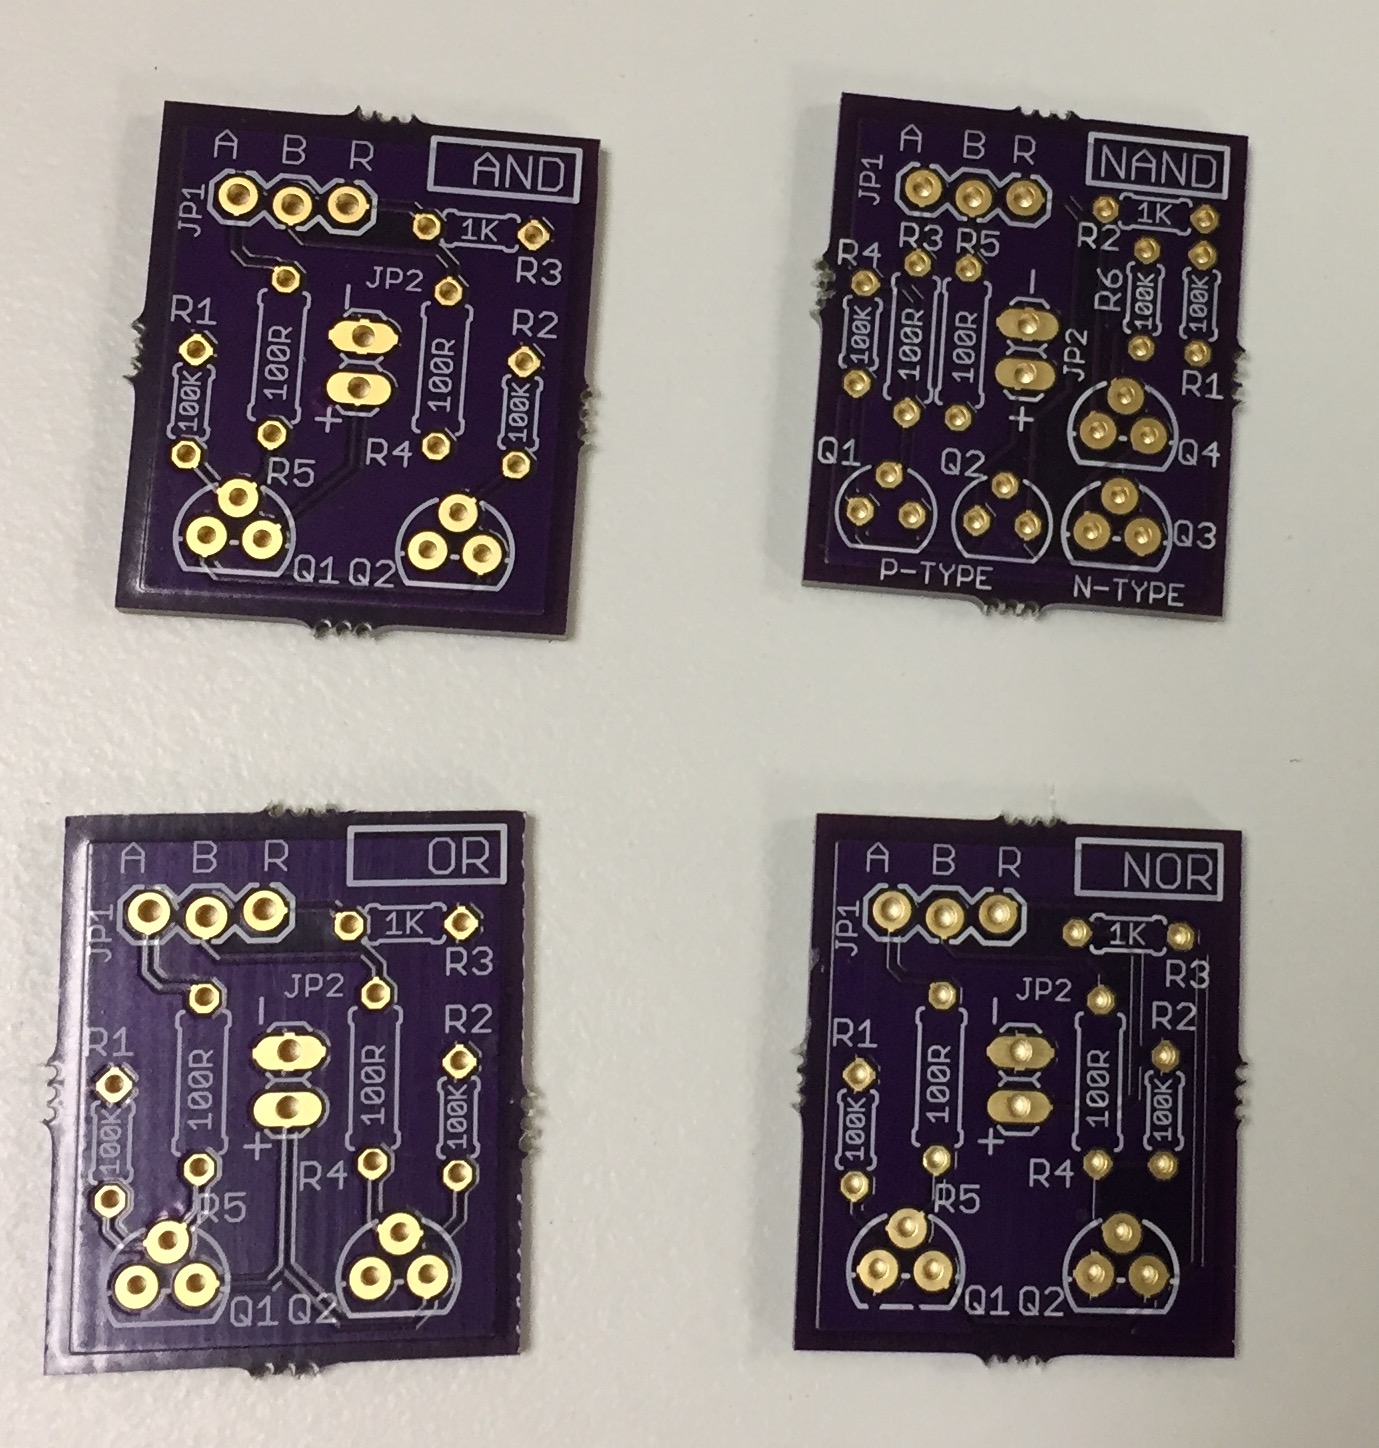
\includegraphics[scale=0.20]{barepcbs.jpg}
}
\end{center}
\caption{Four of the bare PCBs you will use when creating the gates. You will solder a set of specific components in the correct places, and then you will end up with the building blocks of computers.}
\label{fig:barepcbs}
\end{figure}

\subsection*{Solder A Simple Gate}

\bi

\+ Get component list 
\+ Identify each resistor by color bands (see Appendix, Figure \ref{fig:resistorchart})
\+ Read part numbers on the transistors to make sure (need magnifying glass)
\+ The transistors are not necessarily the same, and transistors \emph{can be put in the wrong way}, so be certain about the orientation of the components before soldering them
\+ Similarly, the values of the resistors matter. Ensure that each resistor matches the value labeled on the circuit board. Some of the resistors have been chosen because they are of different sizes and colors, but the bands on the resistor are the best way to check the component
\+ Bending the resistor leads tightly is a challenge for small and inexperienced hands: the best way is to pinch the resistor body close to the lead, and place the index finger of the other hand at the joint where the lead meets the resistor body. Then, ``roll'' the finger, pressing tightly the whole time, such that the lead stays close to the body but ends up perpendicular to the body.
\+ If resistor leads aren't quite tightly bent, use pliers on the underside of the PCB to pull the resistor down into place.
\+ Resistors should be flat against the circuit board!
\+ Solder resistors first
\+ Then solder the transistors
\+ Lastly, solder the headers (note: it may be helpful to use headers with long pins on both sides, to enable both breadboard use and discrete-wiring use, but otherwise solder the headers with the long pins facing \emph{down})
\+ Soldering the headers may be easier if the headers are put in place on a solderless breadboard, with the gate PCB laid on top of them, and then soldered in place. \emph{Caution:} if you take too long to solder the headers this way, the heat can begin to melt the plastic body of the solderless breadboard.
\+ Always test each gate to ensure that it works. Occasional errors (even in the PCB manufacturing process!) can be frustrating, and it's easier to catch these errors while the iron is literally hot

\ei

\pagebreak
This project includes a separate {\color{webblue}\href{https://github.com/jessehamner/TechMillForKids/tree/master/soldering}{PDF project}} that teaches basic through-hole soldering. \emph{Because soldering irons get very hot, adult supervision and safety glasses are required.}

\begin{figure}[hb!]
\begin{center}
\fbox{
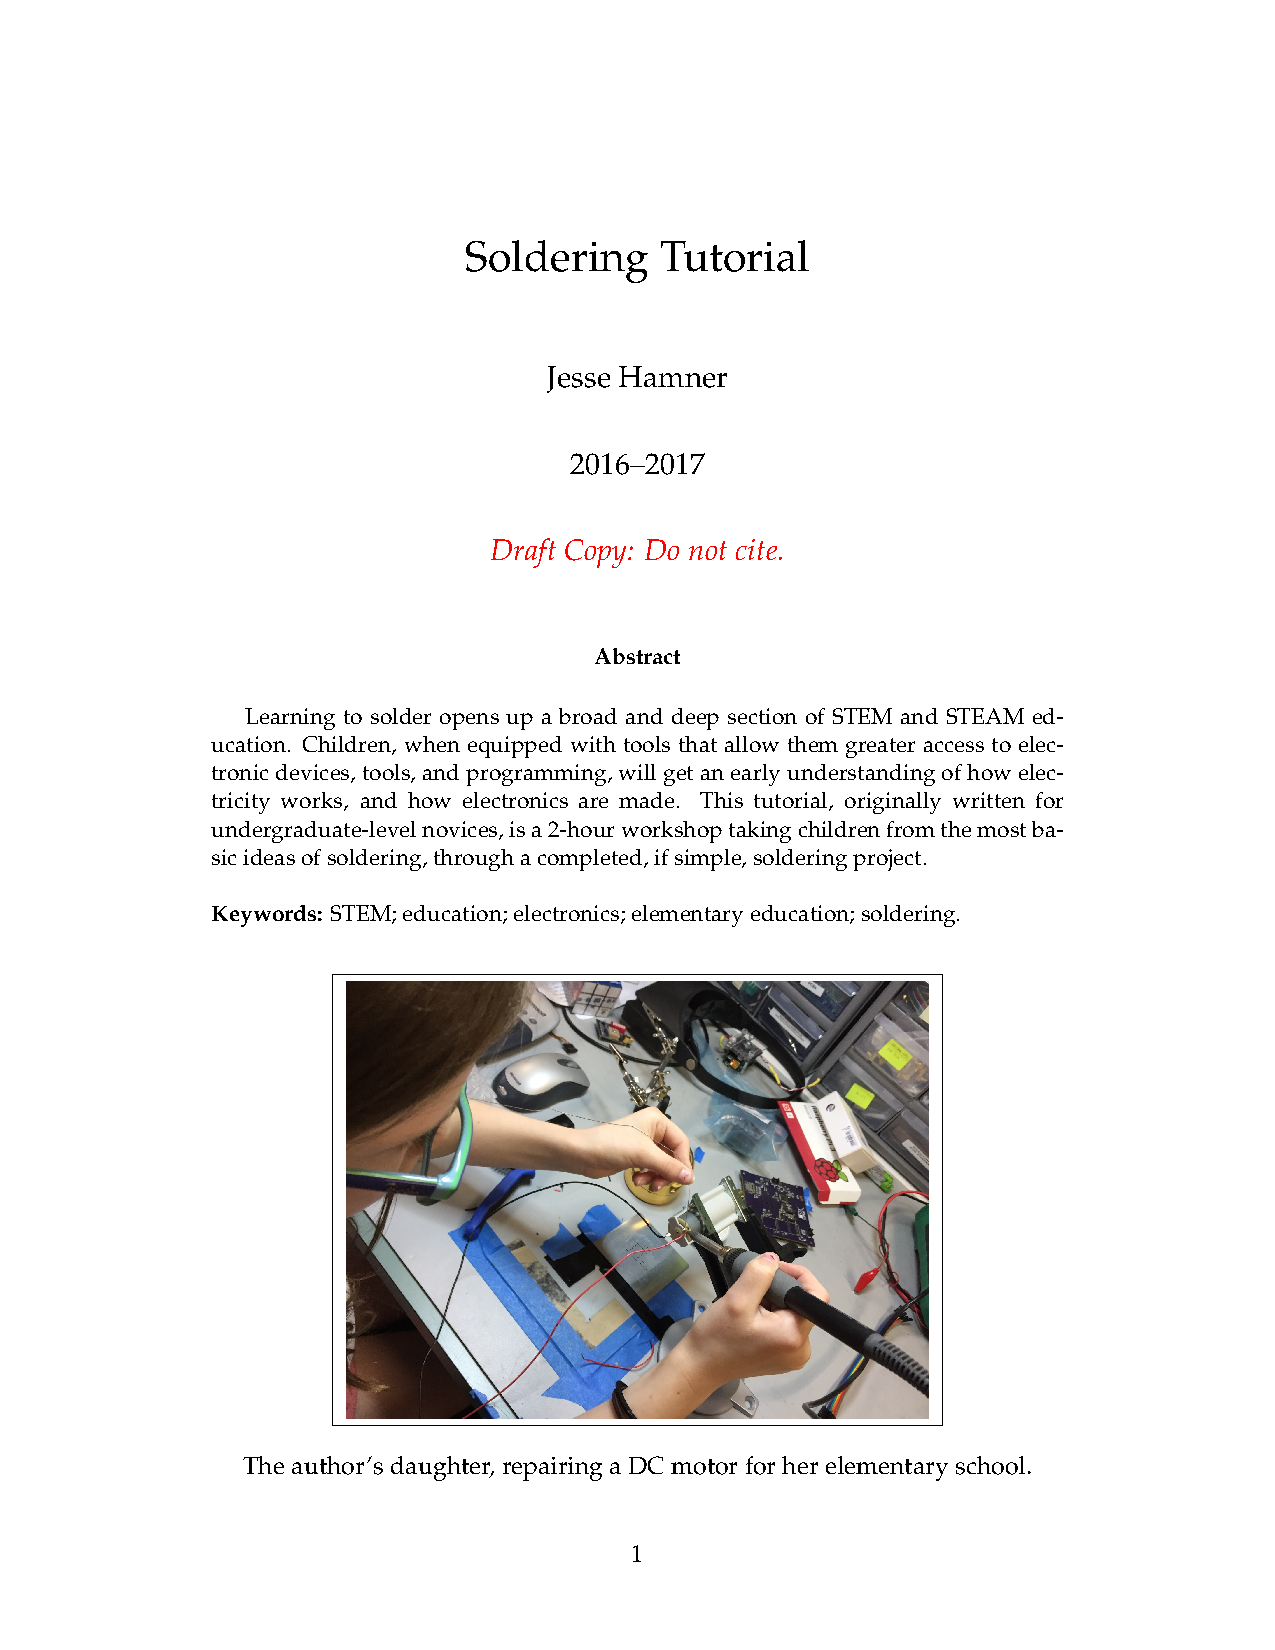
\includegraphics[scale=0.40,origin=c,
	clip=true, trim=80 60 80 110, page=1]{SolderTutorial.pdf}
}
\end{center}
\caption{The soldering tutorial PDF front page.}
\label{fig:soldering}
\end{figure}

\begin{figure}[hb!]
\begin{center}
\fbox{
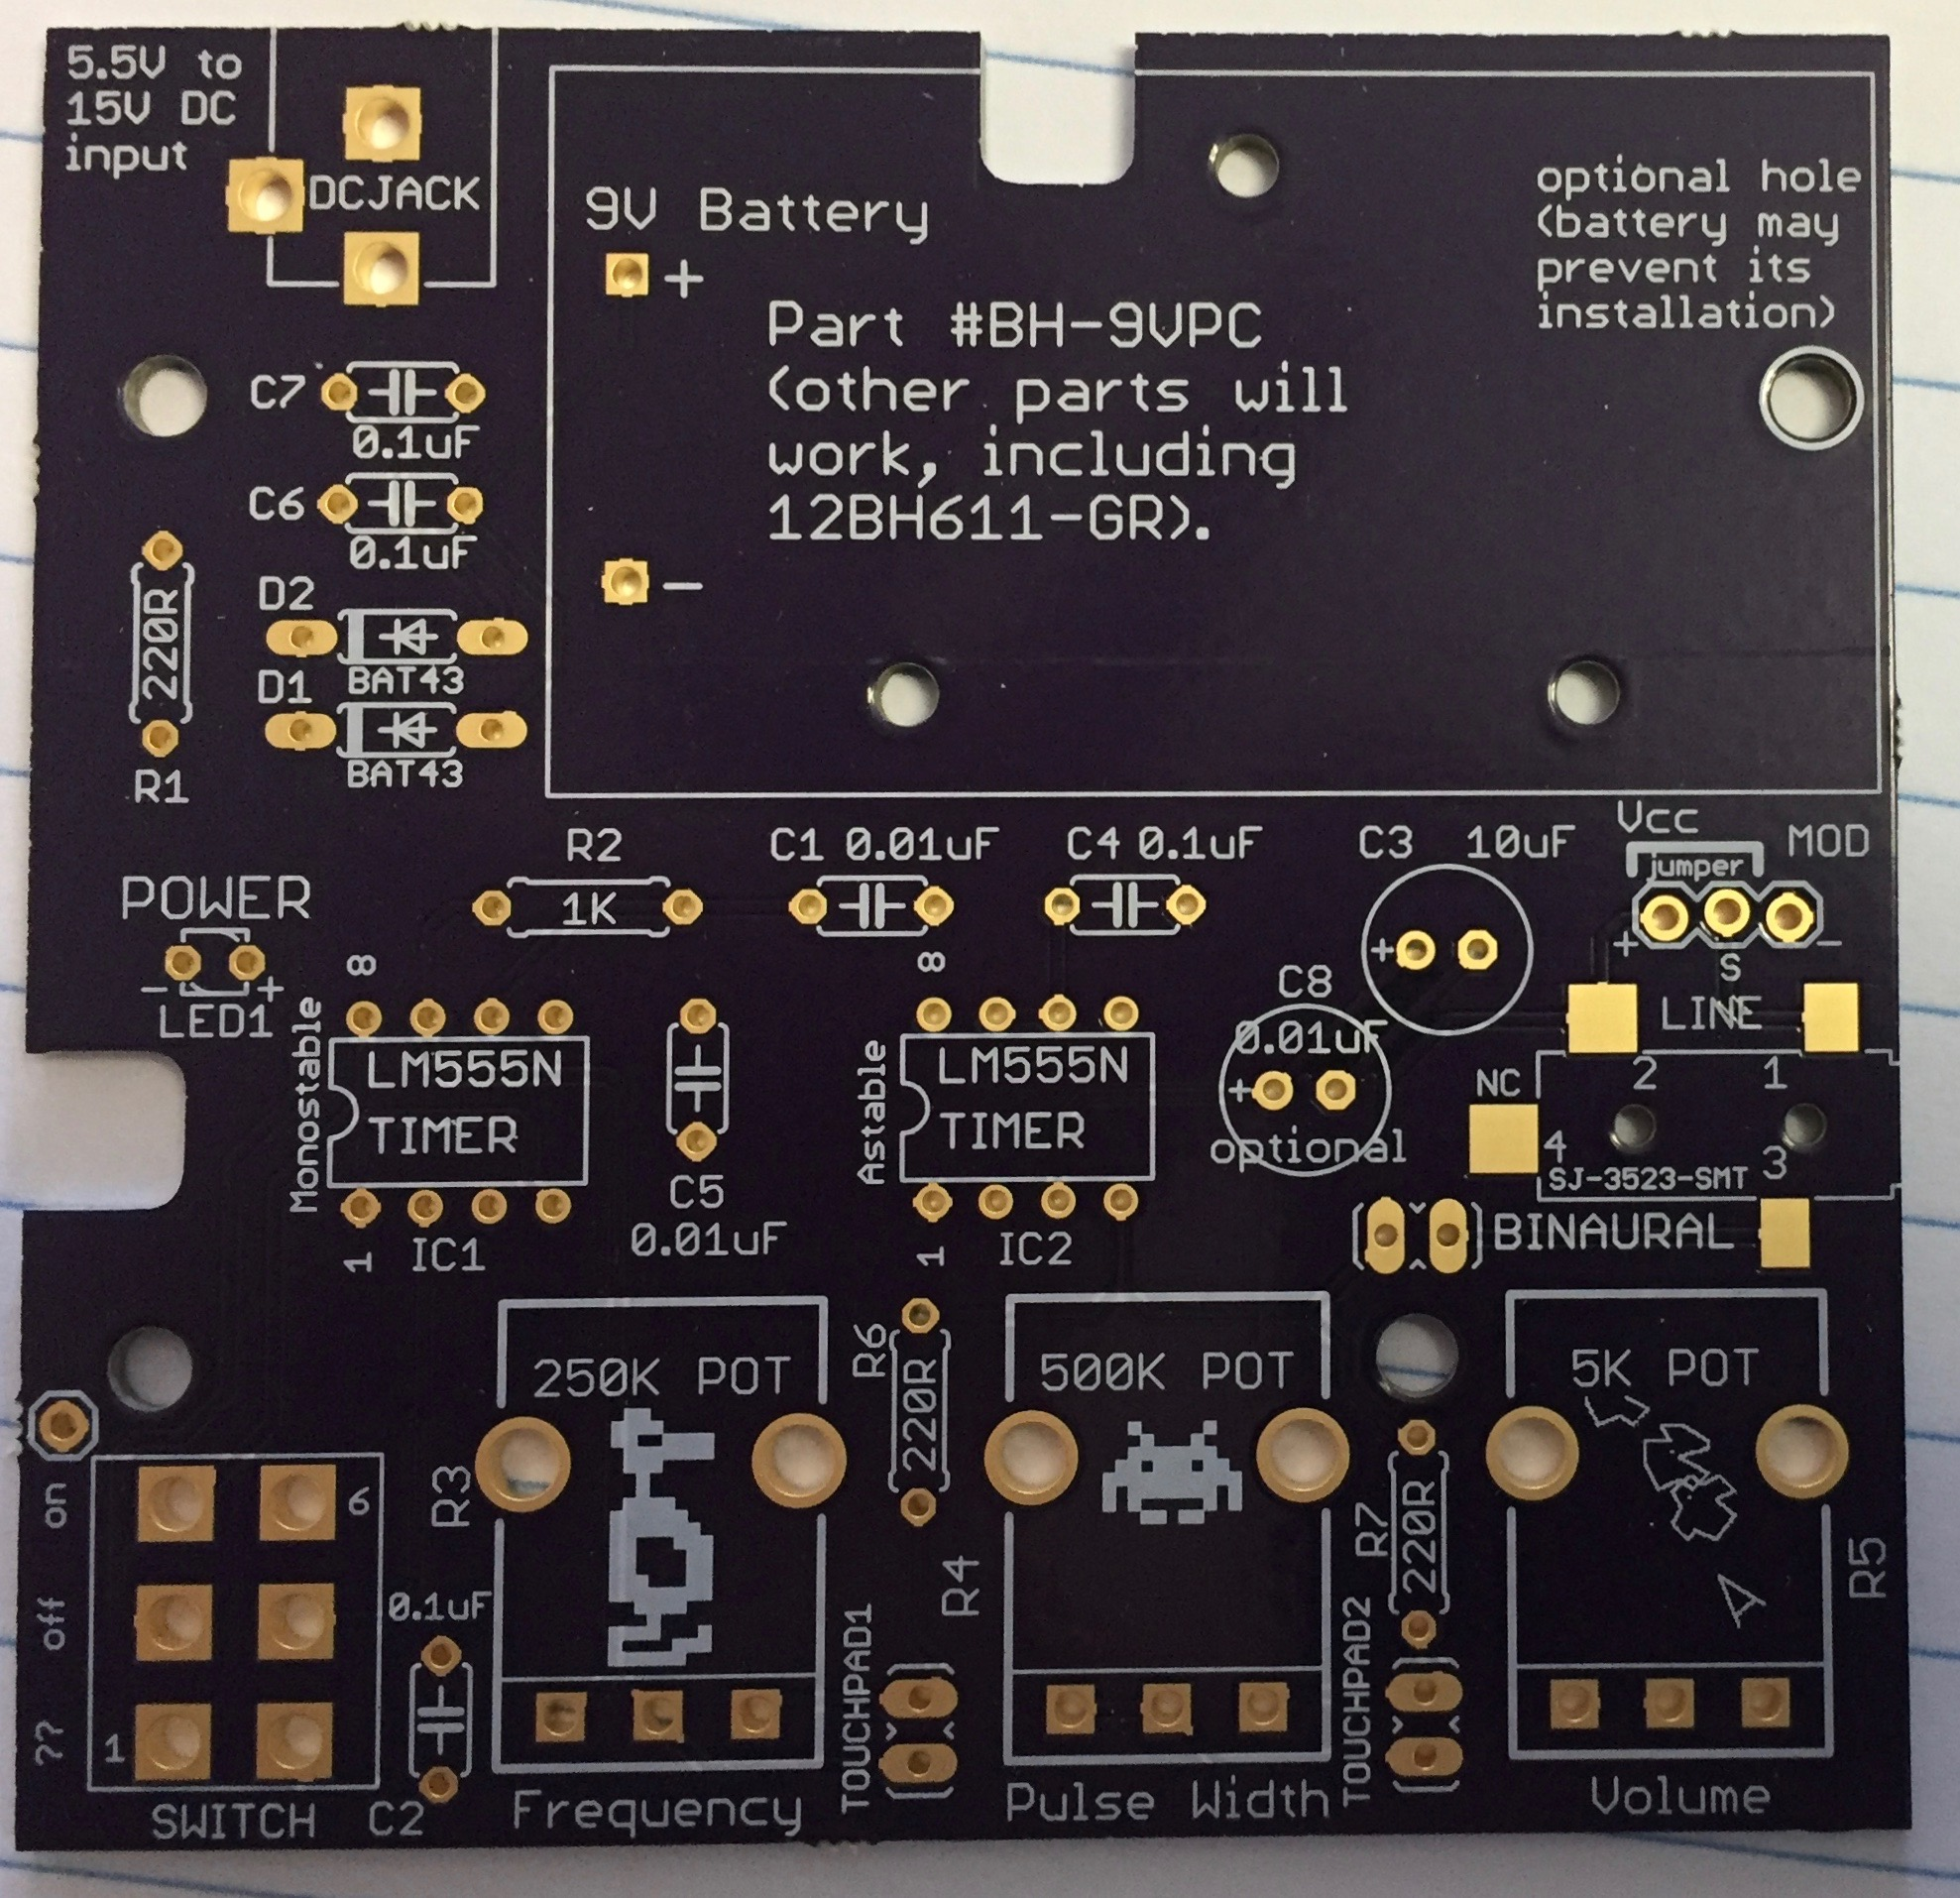
\includegraphics[scale=0.09]{PCB.jpg}
}
\end{center}
\caption{For even more soldering (but still made for beginners), check out the {\color{webblue}\href{https://github.com/jessehamner/AtariPunkConsole}{Atari Punk Console project}}.}
\label{fig:soldering}
\end{figure} 

\clearpage